\documentclass{templateNote}
\usepackage{tcolorbox}
\usepackage{xcolor}
\usepackage{amssymb}
\usepackage{pgfplots}
\usepackage{tikz}

\newcommand{\destacar}[1]{ \colorbox{yellow}{#1}}

\begin{document}

\imagenlogo{img/logoUBB.png}
\universidad{Universidad del Bío-Bío pepito5}
\titulo{Apunte Economia} % Titulo
\asignatura{Economia 1} % Asignatura
\autor{
    \indent
    Marcelo \textsc{Paz}
}
\portada
\margenes % Crear márgenes

\section{Importante}
\begin{itemize}
    \item \textbf{Felicidad:} Es la satisfacción de las necesidades. (Siempre que puedas vas a querer más).
    
    \item \textbf{Ceteris paribus:} Las variables que no se están estudiando, se asumen constante (no varían) durante el periodo estudiado. En otras palabras, \destacar{las demás cosas se mantienen} \destacar{constantes/iguales}.

    \item \textbf{Funcion de Demanda:} 
    \begin{align*}
        {Q_x}^d = f(P_x, P_y, Y, G, E)
    \end{align*}
* ${Q_x}^d$ = Cantidad demandada de $x$.\\
* $P_x$ = Precio de $x$.\\
* $P_y$ = Precio de $y$.\\
* $Y$ = Ingreso del consumidor.\\
* $G$ = Gustos del consumidor.\\
    
    \item \textbf{Funcion de Oferta:}
    \begin{align*}
        {Q_x}^s = f(P_x, P_y, P_f, T, E)
    \end{align*}
* ${Q_x}^s$ = Cantidad ofrecida de $x$.\\
* $P_x$ = Precio de $x$.\\
* $P_y$ = Precio de $y$.\\
* $P_f$ = Precio de los factores.\\
* $T$ = Tecnología.\\
* $E$ = Expectativas.\\

    \item \textbf{Equilibrio de mercado:} Es el punto de intersección entre la curva de oferta y la curva de demanda.\\
    \begin{align*}
        {Q_x}^d = {Q_x}^s
    \end{align*}
    
    \item \textbf{Relación de preferencia:}
    \begin{itemize}
        \item $A \succsim B$ (A es preferido o indiferente a B)
        \item $A \succ B$ (A es preferido a B)
        \item $A \sim B$ (A es indiferente a B)
    \end{itemize}

    \item \textbf{Axiomas de la teoría del consumidor:}
    \begin{enumerate}
        \item Las preferencias son \textbf{completas:}
        \begin{itemize}
            \item \destacar{Se refiere a que los individuos son capaces de tomar sus propias decisiones.}
            \item Cuando un consumidor se enfrenta a una elección entre dos grupos de
            bienes (A y B),puede clasificarlos de modo que $A \succsim B$, $B \succsim A$ o $A \sim B$.
            \item El consumidor puede comparar cualquier par de cestas.
        \end{itemize}

        \item Las preferencias son \textbf{transitivas}
        \begin{itemize}
            \item \destacar{El consumidor tiene la capacidad de jerarquizar sus preferencias.}
            \item Las clasificaciones de los consumidores son lógicamente consistentes en
            el sentido de que si $A \succsim B$ y $B \succsim C$, entonces $A \succsim C$.
            \item Esta propiedad evita la existencia de ciclos, $A \succ B \succ C \succ A$.
        \end{itemize}
        \item Las preferencias son \textbf{monótonas}
        \begin{itemize}
            \item \destacar{El consumidor siempre va a preferir lo que de mayor utilidada.}
            \item Sea $A = (x,y)$, $B = (x',y')$: \\
            $x \geq  x'$, $y \geq y'$ implica $A \succsim B$.
            $x >  x'$, $y > y'$ implica $A \succ B$.
            \item El bienestar del consumidor aumentó si tiene más de cualquier bien.
        \end{itemize}

    \end{enumerate}

    \item \textbf{Curva de indiferencia:} Es una curva que representa todas las combinaciones de dos bienes que proporcionan al consumidor el mismo nivel de satisfacción o utilidad.\\
    Propiedades:
    \begin{enumerate}
        \item Se prefieren los grupos de bienes en las curvas de indiferencia más
        alejados del origen a los de las curvas de indiferencia más cerca del
        origen.
        
        \item Cada paquete se encuentra en una curva de indiferencia.
        
        \item Las curvas de indiferencia no se pueden cruzar.

        \item Las curvas de indiferencia no pueden tener pendiente positiva.
        
        \item Las curvas de indiferencia no pueden ser gruesas.
    \end{enumerate}

    \item \textbf{Funcion de Utilidad:} Es una función que asigna un número a cada cesta de consumo, de tal forma que las cestas con mayor utilidad tienen un número mayor.
    \begin{align*}
        U(q_1,q_2) 
    \end{align*}
    Permite la comparación de los conjuntos:    
    \begin{align*}
        U(x) > U(y) \quad \text{es equivalente a} x \succ y \\
        U(x) = U(y) \quad \text{es equivalente a} x \sim y
    \end{align*}
    
    \begin{itemize}
        \item \textbf{Ordinal:} Ayuda al orden.
        \item \textbf{Cardinal:} Nos ayuda a conocer con exactitud el valor de los bienes y compararlos. Tambien permite obtener la utilidad marginal.
    \end{itemize}
    \item \textbf{Utilidad Marginal:} Es el cambio en la utilidad total que se produce al aumentar en una unidad la cantidad consumida de un bien, manteniendo constante la cantidad consumida de los demás bienes.
    \begin{align*}
        U_m &= \frac{\Delta U}{\Delta x} \quad \textbf{, discreta} \quad U_m = \frac{\mathrm{d} U}{\mathrm{d}x} \quad \textbf{, continua}
    \end{align*}

    \item \textbf{Tasa margial de sustitución (TMS):} Es la tasa a la que un consumidor está dispuesto a cambiar un bien por otro, manteniendo el mismo nivel de utilidad.\\
    \begin{equation*}
        TMS =- \frac{U_1}{U_2} = \frac{\mathrm{d} q_2}{\mathrm{d} q_1} = - \left(\frac{\partial U}{\partial q_1} / \frac{\partial U}{\partial q_2}\right) 
    \end{equation*}

    \item \textbf{Tasa marginal de transformación (TMT):} Es la tasa a la que un consumidor puede cambiar un bien por otro, manteniendo el mismo nivel de utilidad.\\
    \begin{equation*}
        TMT =- \frac{p_1}{p_2}
    \end{equation*}

    \item \textbf{Formula del Ingreso:} $p_1 q_1 + p_2 q_2 = Y$
    
    \item \textbf{Maximizacion de utilidad del consumidor:} Cuando la utilidad marginal es igual al precio.
    \begin{align*}
        - \frac{U_1}{U_2} = - \frac{p_1}{p_2}
    \end{align*}
    
    \item \textbf{Problema de maximización:} Es el proceso de encontrar la mejor solución, entre todas las posibles, para un problema dado. Es decir, el proceso de encontrar el máximo o mínimo de una función, llamada función objetivo, sujeta a un conjunto de restricciones.
    \begin{align*}
        max_{q_1, q_2} (U(q_1,q_2)) \\
        \text{s.a.} \quad p_1 q_1 + p_2 q_2 = Y
    \end{align*}
    
    \item \textbf{Método de sustitución:} Es un método para resolver problemas de optimización de dos variables.\\
    \begin{itemize}
        \item \textbf{Paso 1:} Despejar una de las variables de la restricción presupuestaria.
        \item \textbf{Paso 2:} Reemplazar la variable despejada en la función de utilidad.
        \item \textbf{Paso 3:} Calcular la condición de primer orden con respecto a la variable que no se despejo.
        \item \textbf{Paso 4:} Despejar la variable que no se despejo en el paso 1.
    \end{itemize}

    \newpage
    \item \textbf{Analisis de estatica comparativa:} Es un método para analizar cómo cambia el equilibrio de un modelo económico cuando cambian los parámetros del modelo.\\
    
    \begin{figure}[H]
        \centering
        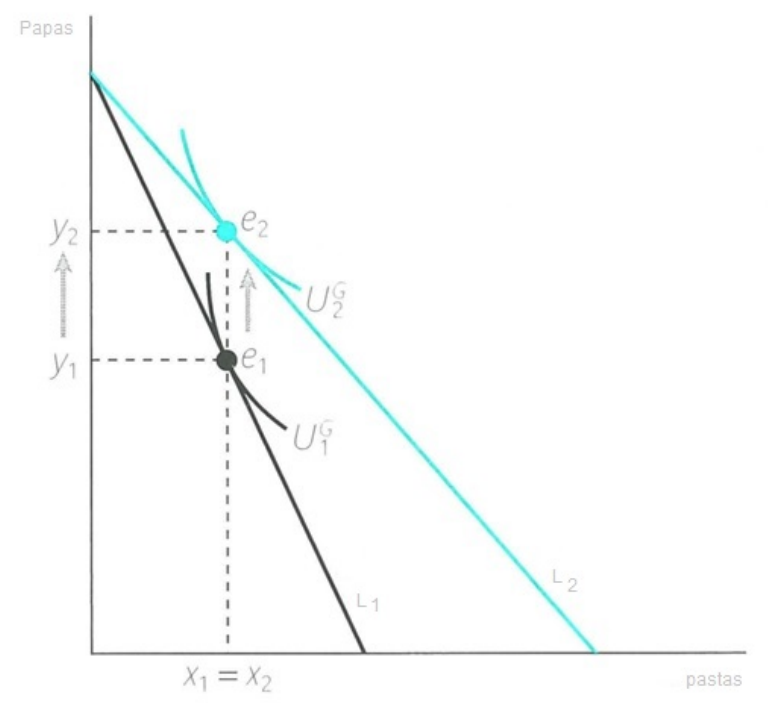
\includegraphics[scale=0.3]{img/Analisis.png}
        \caption{Analisis de estatica comparativa}
    \end{figure}

    \item \textbf{Curva de Engel:} Es una curva que muestra la relación entre la cantidad demandada de un bien y el ingreso del consumidor, manteniendo constante el precio del bien y los precios de los demás bienes.\\
    \begin{figure}[H]
        \centering
        \begin{tikzpicture}
            \begin{axis}[ 
                axis lines = left,
                xlabel style={at={(rel axis cs:1.04,0)}, anchor=west},
                ylabel style={rotate =-90 ,at={(rel axis cs:0.10,1.03)}, anchor=south},
                xmax = 10,
                ymax = 10,
                height = 10cm,
                width = 10cm,
                xmin = 0,
                ymin = 0,
                xlabel = $q_x$,
                ylabel = $Y$,
            ]
            \addplot [
                domain=0:10, 
                samples=100, 
                color=red,
            ]
            {x^2/5};
            \addplot [
                domain=0:4, 
                dashed,
                samples=100, 
                color=blue,
            ]
            {16/5};
            \addplot [
            domain=0:16/5,
            dashed,
            samples=100,
            color=blue
            ] coordinates {(4, 0) (4, 16/5)};
            \addplot [
                domain=0:6, 
                dashed,
                samples=100, 
                color=blue,
            ]
            {36/5};
            \addplot [
            domain=0:36/5,
            dashed,
            samples=100,
            color=blue
            ] coordinates {(6, 0) (6, 36/5)};
            \draw (axis cs:4,3.5) node[above] {${E_1}^*$};
            \draw (axis cs:6,7.7) node[above] {${E_2}^*$};
            \addlegendentry{$q_x = Y$}
            \end{axis}
        \end{tikzpicture}
        \caption{Curva de Engel}
    \end{figure}

    \newpage
    \item \textbf{Elasticidad:} El cambio porcentual en una variable debido a un cambio porcentual en
    otra variable.
    \begin{itemize}
        \item \textbf{Elasticidad precio de la demanda:}
        \begin{align*}
            \mathcal{E}_D &= \frac{\%\Delta q}{\%\Delta p} \\
            \mathcal{E}_D &= \displaystyle \frac{100 \times \left[\frac{q_{nuevo} - q_{previo}}{q_{previo}}\right]}{100 \times \left[\frac{p_{nuevo} - p_{previo}}{p_{previo}}\right]} \\
            \mathcal{E}_D &= \frac{\Delta q/q}{\Delta p/p} \\
            \mathcal{E}_D &= \frac{\partial q}{\partial p} \frac{p}{q}
        \end{align*}
        * Donde $\Delta q = q_{nuevo} - q_{previo}$ y $q = q_{previo}$ \\
        * Donde $\Delta p = p_{nuevo} - p_{previo}$ y $p = p_{previo}$

        \textbf{Los bienes tienen una demanda:}
        \begin{itemize}
            \item $ 0 > \mathcal{E}_D > -1$: Inelástica.
            \item $ \mathcal{E}_D = 1$: Elasticidad unitaria.
            \item $ \mathcal{E}_D < -1$: Elástica.
        \end{itemize}

        \item \textbf{Elasticidad renta de la demanda:}
        \begin{align*}
            \mathcal{E}_Y = \frac{\partial q}{\partial Y} \frac{Y}{q}
        \end{align*}
        \begin{itemize}
            \item $ \mathcal{E}_Y > 0 $: Bien normal.
            \item $ \mathcal{E}_Y < 0 $: Bien inferior.
            \item $ \mathcal{E}_Y > 1 $: Bien de lujo.
        \end{itemize}

        \item \textbf{Elasticidad precio cruzado de la demanda:}
        \begin{align*}
            \mathcal{E}_{AB} = \frac{\partial q_A}{\partial p_B} \frac{p_B}{q_A}
        \end{align*}
        \begin{itemize}
            \item $ \mathcal{E}_{AB} > 0 $: Bienes sustitutos en demanda.
            \item $ \mathcal{E}_{AB} < 0 $: Bienes complementarios en demanda.
        \end{itemize}

        \item \textbf{Elasticidad precio de la oferta:}
        \begin{align*}
            \mathcal{E}_o = \frac{\% \text{cambio en la cantidad ofrecida}}{\% \text{cambio en el precio}} \frac{p}{q}
            \mathcal{E}_o = \frac{\partial q}{\partial p} \frac{p}{q}
        \end{align*}
    \end{itemize}
    \item 
    \section*{Falta clase 8}
\end{itemize}

% \newpage
% \section*{Clase 1}
% \section{Conceptos básicos}
% \begin{enumerate}
%     \item \textbf{Economía:} Es la ciencia que estudia la forma en que los individuos y la sociedad efectúan las elecciones y decisiones para lograr el mejor uso posible de los recursos escasos, que tienen usos alternativos, para satisfacer sus necesidades ilimitadas.\\
    
%     Enfoque de:
%     \begin{enumerate}
%         \item \textbf{Microeconómico:} estudia los comportamientos básicos de los
%         agentes económicos individuales.
%         \item \textbf{Macroeconómico:} analiza comportamientos agregados o
%         globales, y se ocupa de temas como el empleo, la inflación o el
%         producto total de una economía.
%     \end{enumerate}
    
% \end{enumerate}

% \section{Microeconomía}
% \indent
% Es la disciplina que estudia la forma en la cual
% se asignan los recursos escasos, entre los diversos usos que
% compiten por ellos, con el proposito de satisfacer parte de los
% deseos ilimitados de los individuos.\\
% Actores:
% \begin{enumerate}
%     \item \textbf{Productores:} Recursos escasos, usos alternativos y múltiples.
%     \item \textbf{Consumidores:} Necesidades múltiples, jerarquizables y progresivas. 
%     \item \textbf{Relación de intercambio.}
% \end{enumerate} 

% \subsection{Aspectos}
% \begin{enumerate}
%     \item Los precios, cantidad, demanda de factores, determinantes del
%     comportamiento.
    
%     \item Fenómenos económicos desagregados de cada agente (empresa,
%     consumidor, etc.) considerando las decisiones que toma cada uno
%     para cumplir ciertos objetivos propios y considerando algunos
%     supuestos de libre empresa o libre mercado.
% \end{enumerate}
% \subsection{Objetivos}
% \begin{enumerate}
%     \item Se considera a la microeconomía como el estudio de la asignación
% de recursos escasos frente a necesidades múltiples.
    
%     \item Uno de los principales objetivos de la microeconomía es analizar
% los mecanismos que establecen los precios relativos de los bienes
% y factores.
    
%     \item La Microeconomía estudia el modo en que toman decisiones los
% hogares y las empresas y la forma en que interactuan.
% \end{enumerate}

% \newpage
% \section{Racionalidad económica}
% \begin{enumerate}
%     \item \textbf{Costo de oportunidad:} Es el \destacar{sacrificio asociado a una decisión.} Se
%     busca maximizar o minimizar su función objetivo, sujeta a
%     restricciones. Por lo general empleamos la matemática para
%     representar estas situaciones.
    
%     \item \textbf{Consumidor:} Su objetivo es \destacar{maximizar la utilidad} derivada del consumo de bienes, sujeta a precios y restricción presupuestaria. \\
% \\
% * Por tanto, el objetivo del consumidor se encuentra en consumir o alcanzar un nivel
% de consumo determinado que nos permita llegar al nivel de utilidad
% o bienestar deseado. \\

%     \item \textbf{Productor:} Su objetivo es \destacar{maximizar los beneficios} (netos) de la producción (máximo ingreso, mínimo costo). \\
% \end{enumerate}
% * \textbf{Modelos económicos:} Es capaz de explicar y predecir los acontecimientos del mundo real (la mejor aproximación).

% \section{Supuestos}
% \begin{enumerate}
%     \item \textbf{Ceteris paribus:} Las variables que no se están estudiando, se
%     asumen constante (no varían) durante el periodo estudiado. En otras palabras, \colorbox{yellow}{las demás cosas se mantienen} 
%     \colorbox{yellow}{constantes/iguales}.

%     \item \textbf{Los agentes} toman decisiones para optimizar algo (maximizar o
%     minimizar).

%     \item \textbf{Distinción entre economía positiva (lo que es) y economía
%     normativa (lo que debería ser).}

%     \item \textbf{Mercado:} Lugar físico o virtual donde se encuentran los compradores y vendedores de un bien o servicio para realizar transacciones comerciales.\\ 
%     \begin{enumerate}
%         \item \textbf{El principio de la optimización:} Los individuos tratan de elegir las
%         mejores pautas de consumo que estan a su alcance.

%         \item \textbf{El principio de equilibrio:} Los precios se ajustan hasta que la
%         cantidad que demanden los individuos de una cosa es igual a la
%         que se ofrece.

%         \item \textbf{El consumidor elige la cesta de consumo} que prefiere dado el
%         conjunto de combinaciones de bienes, y la optimización que
%         puede alcanzar.

%         \item \textbf{Los consumidores tienen preferencias} sobre algunos bienes y servicios.
        
%     \end{enumerate}
% * Lo anterior se refiere a que los consumidores, dados los precios
% de estos bienes preferirán una canasta sobre la otra.
% \end{enumerate}

% \section{Montaña de la felicidad}
% \indent

% La montaña de la felicidad es una representación gráfica de las preferencias de un individuo.\\
% \begin{itemize}
%     \item Donde $U_5$ es la mayor utilidad y $U_1$ la menor utilidad.
%     \item Cada nivel esta limitado por la restricción presupuestaria.
% \end{itemize}

% \begin{equation*}
%     U_5 > U_4 > U_3 > U_2 > U_1
% \end{equation*}

% \begin{figure}[H]
%     \centering
%     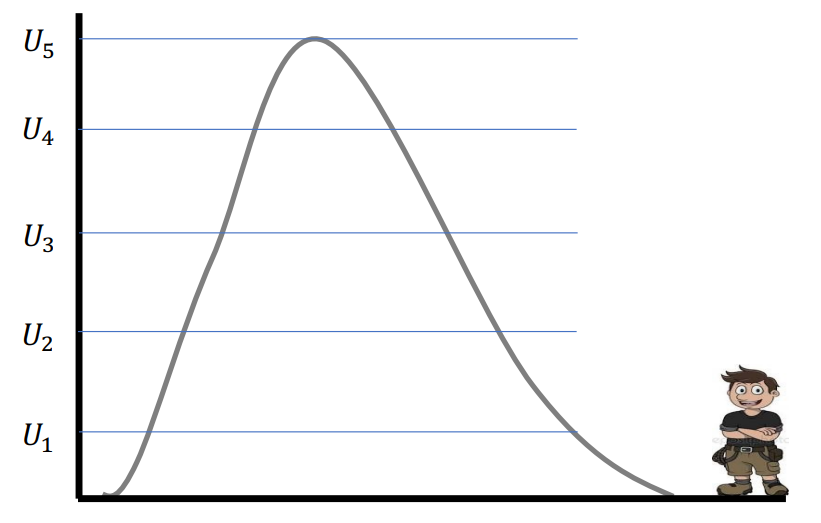
\includegraphics[scale=0.5]{img/Mountain.png}
%     \caption{Montaña de la felicidad}
% \end{figure}

% \section{Mercado}

% \begin{enumerate}
%     \item \textbf{Monopolio(único vendedor):}Es una estructura de mercado
%     caracterizada por la presencia de una \destacar{única empresa}, que
%     produce un bien homogéneo y que \destacar{define sus precios}, calidad,
%     cantidad y mercado.

%     \item \textbf{Competencia perfecta:}
%     \begin{itemize}
%         \item Aquella en que hay varios productores que \destacar{compiten en igualdad
%         de condiciones} para atraer la demanda de los consumidores.

%         \item Una economía liberal es el sistema ideal de desarrollo para los
%         mercados y lograr satisfacer al consumidor
%     \end{itemize}

% \newpage
%     \item \textbf{Oligopolio:}
%     \begin{itemize}
%         \item Del griego, pocos vendedores. \destacar{Se supone que hay pocas
%         empresas, pero de tal} \destacar{forma que, ninguna de ellas puede
%         controlar totalmente el mercado.}

%         \item Hay por ello una constante lucha entre las mismas, para poder
%         llevarse la mayor parte de la cuota de mercado.

%         \item Así las empresas toman decisiones estratégicas, teniendo
%         encuenta las fortalezas y debilidades de la estructura empresarial
%         de cada una.        
%     \end{itemize}

%     \item \textbf{Competencia monopolística:}
%     \begin{itemize}
%         \item Es una estructura de mercado caracterizada por la presencia de
%         muchas empresas que venden productos homogéneos,
%         sustitutivos cercanos, pero distintos, entre sí.

%         \item Al tratarse de productos heterogéneos, cada productor tiene un
%         cierto poder de mercado sobre el bien que produce, por lo que la
%         competencia monopolística puede definirse como una estructura
%         de mercado intermedia entre monopolio en competencia
%         perfecta.
%     \end{itemize}
% \end{enumerate}

% \section{Grandes Interrogantes}
% \subsection{¿Qué y cuánto producir?}
% \indent
% Elección de bienes y servicios a ofertar según las necesidades.

% \subsection{¿Cómo producir?}
% \indent
% Elección de la forma a utilizar para transformar los bienes.

% \subsection{¿Para quién producir?}
% \indent
% Decidir sobre la distribución de la producción entre los individuos.

\newpage
\section{Ejercicios}
\subsection{Problema de maximización visto en clase}
\begin{itemize}
    \item Sea la función de utilidad $U(q_1,q_2) = q_1 \cdot q_2$
    \item La renta $Y = 200$.
    \item Los precios $p_1 = 4$ y $p_2 = 1$.
\end{itemize}

Entonces:
\begin{equation*}
    \begin{split}
        max_{q_1, q_2} (q_1 \cdot q_2) \\
        \text{s.a.} \quad 4q_1 + q_2 = 200 \\
    \end{split}
\end{equation*}
* s.a. = sujeto a.\\
\begin{itemize}
    \item \textbf{Paso 1:} Resolver la restricción de presupuesto para $q_2$.
    \begin{align*}
        q_2 &= 200 -4q_1
    \end{align*}
    
    \item \textbf{Paso 2:} Reemplazar la restricción en la función de utilidad.
    \begin{align*}
        max_{q_1} (q_1 \cdot (200 -4q_1)) &= q_1 \cdot (200 -4q_1) \\
        &= 200q_1 -4 {q_1}^2
    \end{align*}
    
    \item \textbf{Paso 3:} Calcular las condiciones de primer orden con respecto a $q_1$.
    \begin{align*}
        \frac{\mathrm{d} U(q_1)}{\mathrm{d}q_1} &= 200 -8q_1 = 0 \Leftrightarrow {q_1}^* = 25
    \end{align*}
    
    \item \textbf{Paso 4:} Utilizar las condiciones de primer orden para despejar $q_2$.
    \begin{align*}
        {q_2}^* &= 200 -4 \times 25 \\
        &= 100 \\
    \end{align*}
    $\therefore \quad$ la utilidad del problema de maximización es:
    \begin{align*}
        U({q_1}^*, {q_2}^*) &= 25 \times 100 \\
        &= 2500
    \end{align*}
    
\end{itemize}

\newpage
\subsection{Material Ayudantia 4}
\subsubsection{Ejercicio 1}
\indent
Explique el paso a paso del Método de Sustitución. Además exprese la ecuación de
optimización y la restricción presupuestaria
\begin{itemize}
    \item \textbf{Paso 1:} Despejar una de las variables de la restricción presupuestaria.
    \item \textbf{Paso 2:} Reemplazar la variable despejada en la función de utilidad.
    \item \textbf{Paso 3:} Calcular la condición de primer orden con respecto a la variable que no se despejo.
    \item \textbf{Paso 4:} Despejar la variable que no se despejo en el paso 1.
    \item \textbf{Paso 5:} Reemplazar el resultado del paso 4 en la restricción presupuestaria para obtener la utilidad máxima.
\end{itemize}

\subsubsection{Ejercicio 2}
\begin{itemize}
    \item Sea la función de utilidad $U(q_1,q_2) = q_1 \cdot q_2$
    \item La renta $Y = 1200$.
    \item Los precios $p_1 = 6$ y $p_2 = 4$.
\end{itemize}

Entonces:
\begin{equation*}
    \begin{split}
        max_{q_1, q_2} (q_1 \cdot q_2) \\
        \text{s.a.} \quad 6q_1 + 4q_2 = 1200
    \end{split}
\end{equation*}
\begin{align*}
    q_2 &= 300 - \frac{3}{2}q_1 \\
    \\
    max_{q_1} (q_1) &= q_1 \cdot (300 - \frac{3}{2}q_1) \\
    &= 300q_1 - \frac{3}{2} {q_1}^2 \\
    \\
    \frac{\mathrm{d} U(q_1)}{\mathrm{d}q_1} &= 300 - 3q_1 = 0 \Leftrightarrow {q_1}^* = 100 \\
    \\
    {q_2}^* &= 300 - \frac{3}{2} \times 100 \\
    &= 150 \\
    \\
    \therefore \quad U({q_1}^*, {q_2}^*) &= 100 \times 150 \\
    &= 15000
\end{align*}

\newpage
\subsubsection{Ejercicio 3}
Suponga que un consumidor cuenta con una renta de 600 unidades monetarias, que puede
gastar únicamente entre dos bienes $A$ y $B$. El precio del bien $A$ es $P_a = 2$, y del bien $B$ es
$P_b = 3$

\textbf{a)} Indique cuál será la función de su restricción presupuestaria.
\begin{align*}
    2A + 3B &= 600
\end{align*}

\textbf{b)} ¿Qué número de unidades del bien $A$ podrá adquirir si dedica toda su renta a
comprar dicho bien?
Sea $B = 0$.
\begin{align*}
    2A + 3(0) &= 2A = 600 \Leftrightarrow A = 300
\end{align*}

\textbf{c)} ¿Cuánto podrá comprar del bien $B$ si no compra nada del bien $A$?
Sea $A = 0$.
\begin{align*}
    2(0) + 3B &= 3B = 600 \Leftrightarrow B = 200
\end{align*}

\textbf{d)} Represente gráficamente la restricción presupuestaria.
\begin{figure}[H]
    \centering
    \begin{tikzpicture}
        \begin{axis}[
            axis lines = left,
            xlabel style={at={(rel axis cs:1.04,0)}, anchor=west},
            ylabel style={rotate =-90 ,at={(rel axis cs:0.10,1.03)}, anchor=south},
            xmax = 500,
            ymax = 350,
            height = 10cm,
            width = 10cm,
            xmin = 0,
            ymin = 0,
            xlabel = $A$,
            ylabel = $B$,
        ]
        \addplot [
            domain=0:300, 
            samples=100, 
            color=red,
        ]
        {200-2/3*x};
        \addlegendentry{$200-\frac{2}{3}A$}
        \end{axis}
    \end{tikzpicture}
    \caption{Restricción presupuestaria}
\end{figure}

\newpage
\textbf{e)}  Si la renta del individuo aumenta hasta hasta $R = 900$, ¿Qué pasaría con la
restricción presupuestaria? Representar gráficamente.

Sea $R = 900$.
\begin{align*}
    2A + 3B &= 900 \\
    3B &= 900 - 2A \\
    B &= 300 - \frac{2}{3}A
\end{align*}

Sea $A = 0$.
\begin{align*}
    B &= 300 - \frac{2}{3} \times 0 \\
    &= 300
\end{align*}

Sea $B = 0$.
\begin{align*}
    2A &= 900 \\
    A &= 450
\end{align*}

\begin{figure}[H]
    \centering
    \begin{tikzpicture}
        \begin{axis}[
            axis lines = left,
            xlabel style={at={(rel axis cs:1.04,0)}, anchor=west},
            ylabel style={rotate =-90 ,at={(rel axis cs:0.10,1.03)}, anchor=south},
            xmax = 500,
            ymax = 350,
            height = 10cm,
            width = 10cm,
            xmin = 0,
            ymin = 0,
            xlabel = $A$,
            ylabel = $B$,
        ]
        \addplot [
            domain=0:300, 
            samples=100, 
            color=red,
        ]
        {200-2/3*x};

        \addplot [
            domain=0:450, 
            samples=100, 
            color=blue,
        ]
        {300-2/3*x};
        \draw[->, thick] (axis cs:160,120) -- (axis cs:230,120);
        \draw (axis cs:175,125) node[above] {$R = 900$};
        \addlegendentry{$200-\frac{2}{3}A$}
        \addlegendentry{$300-\frac{2}{3}A$}
        \end{axis}
    \end{tikzpicture}
    \caption{Restricción presupuestaria}
\end{figure}

\newpage
\textbf{f)} Suponga ahora que, en lugar del incremento de la renta, el precio del bien $A$ se
duplica. Represente la nueva restricción presupuestaria.

Sea $P_a = 4$.
\begin{align*}
    4A + 3B &= 600 \\
    3B &= 600 - 4A \\
    B &= 200 - \frac{4}{3}A
\end{align*}

Sea $A = 0$.
\begin{align*}
    B &= 200 - \frac{4}{3} \times 0 \\
    &= 200
\end{align*}

Sea $B = 0$.
\begin{align*}
    4A &= 600 \\
    A &= 150
\end{align*}

\begin{figure}[H]
    \centering
    \begin{tikzpicture}
        \begin{axis}[
            axis lines = left,
            xlabel style={at={(rel axis cs:1.04,0)}, anchor=west},
            ylabel style={rotate =-90 ,at={(rel axis cs:0.10,1.03)}, anchor=south},
            xmax = 350,
            ymax = 250,
            height = 10cm,
            width = 10cm,
            xmin = 0,
            ymin = 0,
            xlabel = $A$,
            ylabel = $B$,
        ]
        \addplot [
            domain=0:300, 
            samples=100, 
            color=red,
        ]
        {200-2/3*x};

        \addplot [
            domain=0:150, 
            samples=100,
            color=blue,
        ]
        {200-4/3*x};
        \draw[<-, thick] (axis cs:110,75) -- (axis cs:160,75);
        \draw (axis cs:120,80) node[above] {$P_a = 4$};
        \addlegendentry{$200-\frac{2}{3}A$}
        \addlegendentry{$200-\frac{4}{3}A$}
        \end{axis}
    \end{tikzpicture}
    \caption{Restricción presupuestaria}
\end{figure}

\newpage
\subsubsection{Ejercicio 4}
\begin{itemize}
    \item Sea la función de utilidad $U(X,Y) = 10 X \cdot Y$
    \item $m = xp_x + yp_y$
    \item Los precios $p_x = 4$ y $p_y = 3$.
    \item La renta $m = 300$.
\end{itemize}

Entonces:
\begin{equation*}
    \begin{split}
        max_{X, Y} (10 X \cdot Y) \\
        \text{s.a.} \quad 4X + 3Y = 300
    \end{split}
\end{equation*}

\begin{align*}
    Y &= 100 - \frac{4}{3}X \\
    \\
    max_{X} (10 X \cdot (100 - \frac{4}{3}X)) &= 1000X - \frac{40}{3} {X}^2 \\
    \\
    \frac{\mathrm{d} U(X)}{\mathrm{d}X} &= 1000 - \frac{80}{3}X = 0 \Leftrightarrow {X}^* = 37,5 \\
    \\
    {Y}^* &= 100 - \frac{4}{3} \times 37,5 \\
    &= 50 \\
    \\
    \therefore \quad U({X}^*, {Y}^*) &= 10 (37,5 \times 50) \\
    &= 18750
\end{align*}

\subsubsection{Ejercicio 5}
\indent
¿En qué caso se maximiza la utilidad del consumidor?

\textbf{R:} Cuando la utilidad marginal es igual al precio.

Cuando la tasa a la que se está dispuesto a cambiar $q_1$ por $q_2$ es igual a la tasa a la que
puedes cambiarlos.

\begin{equation*}
    TMS = TMT \Leftrightarrow - \frac{U_1}{U_2} = - \frac{p_1}{p_2} \Leftrightarrow \frac{U_1}{U_2} = \frac{p_1}{p_2}
\end{equation*}
* \textbf{TMS} = Tasa marginal de sustitución.\\
* \textbf{TMT} = Tasa marginal de transformación.\\
* $\mathbf{U_1}$ = Utilidad marginal de $q_1$.\\
* $\mathbf{U_2}$ = Utilidad marginal de $q_2$.\\
* $\mathbf{p_1}$ = Precio de $q_1$.\\
* $\mathbf{p_2}$ = Precio de $q_2$.\\

\newpage
\subsection{Material Ayudantia 2}
\subsubsection{Ejercicio 1}
\indent
La demanda por libros es: $P = 200 -0.2x$

\textbf{a)} ¿Cuál es la cantidad consumida al precio de \$50?

Sea $P = 50$.
\begin{align*}
    P &= 200 -0.2x \\
    50 &= 200 -0.2x \\
    0.2x &= 150 \\
    x &= 750
\end{align*}

\textbf{b)} ¿Cuál es el excedente de los consumidores?

\textbf{Calculo de excedente visto en clases:}
\begin{align*}
    EC &= {P_1}_{max} - {P_1}_{actual} \\
    &= 200 -50 \\
    &= 150
\end{align*}
* ${P_1}_{max}$ = Precio máximo. $Q_1$ = 0\\
* ${P_1}_{equilibrio}$ = Precio actual. $Q_1$ = 50\\ 

\textbf{Calculo de excedente visto en internet:}
\begin{align*}
    EC &= \int_{0}^{750} (200 -0.2x) \mathrm{d}x \\
    &= 200x -0.1 {x}^2 \Big|_{0}^{750} \\
    &= 200(750) -0.1 {750}^2 - 0 \\
    &= 112500 - 56250 \\
    &= 56250
\end{align*}

\textbf{c)} Si el precio se reduce a \$40, ¿Cuál es el cambio del excedente?

Sea $P = 40$.

\textbf{Calculo de excedente visto en clases:}
\begin{align*}
    CS &= {P_1}_{max} - {P_1}_{actual} \\
    &= 200 -40 \\
    &= 160
\end{align*}
* ${P_1}_{max}$ = Precio máximo. $Q_1$ = 0\\
* ${P_1}_{equilibrio}$ = Precio actual. $Q_1$ = 40\\

\newpage
\subsubsection{Ejercicio 2}
Suponga la siguiente curva de demanda para el bien $X = 110 - 2P$, donde $P$ es el precio
por unidad del bien, y X son las unidades del bien mensuales.

\textbf{a)} Determine cuánto será la cantidad demandada del bien, a un precio de \$20 la
unidad. Grafique

Sea $P = 20$.
\begin{align*}
    X &= 110 -2(20) \\
    &= 110 -40 \\
    &= 70
\end{align*}

\begin{figure}[H]
    \centering
    \begin{tikzpicture}
        \begin{axis}[
            axis lines = left,
            xlabel style={at={(rel axis cs:1.04,0)}, anchor=west},
            ylabel style={rotate =-90 ,at={(rel axis cs:0.10,1.03)}, anchor=south},
            xmax = 60,
            ymax = 120,
            height = 10cm,
            width = 10cm,
            xmin = 0,
            ymin = 0,
            xlabel = $P$,
            ylabel = $X$,
        ]
        \addplot [
            domain=0:60, 
            samples=100, 
            color=red,
        ]
        {110-2*x};

        \addplot [
            domain=0:20, 
            dash pattern=on 10pt,
            samples=100,
            color=blue
        ] coordinates {(0, 70) (20, 70)};
        
        \draw (axis cs:24,70) node[above] {($20, 70$)};
        
        \addplot [
            domain=0:20,
            dash pattern=on 10pt,
            samples=100,
            color=blue
        ] coordinates {(20, 0) (20, 70)};
        
        \draw[fill = black] (axis cs:20, 70) circle[radius=2pt];
        
        \addlegendentry{$110-2P$}
        
    \end{axis}
    \end{tikzpicture}
    \caption{Curva de demanda para $P_{equilibrio}$}
\end{figure}

\newpage
\textbf{b)} ¿Qué ocurre con la demanda si el ingreso del consumidor se incrementa, ceteris
paribus, y le permite demandar 4 unidades más a un precio de \$20 y un \$22?.
Grafique

Sea $P = 20$ y $X = 114 -2(P)$\\
\begin{align*}
    X &= 114 -2(20)\\
    &= 114 -40\\
    &= 74
\end{align*}

Entonces para $P = 22$.
\begin{align*}
    X &= 114 -2(22) \\
    &= 114 -44 \\
    &= 70
\end{align*}

\begin{figure}[H]
    \centering
    \begin{tikzpicture}
        \begin{axis}[
            axis lines = left,
            xlabel style={at={(rel axis cs:1.04,0)}, anchor=west},
            ylabel style={rotate =-90 ,at={(rel axis cs:0.10,1.03)}, anchor=south},
            xmax = 60,
            ymax = 120,
            height = 10cm,
            width = 10cm,
            xmin = 0,
            ymin = 0,
            xlabel = $P$,
            ylabel = $X$,
        ]
        \addplot [
            domain=0:60, 
            samples=100, 
            color=red,
        ]
        {110-2*x};

        \addplot [
            domain=0:60, 
            samples=100, 
            color=green,
        ]
        {114-2*x};
        
        \draw[fill = black] (axis cs:20, 74) circle[radius=2pt];
        \draw[fill = black] (axis cs:22, 70) circle[radius=2pt];
        
        \addlegendentry{$110-2P$}
        \addlegendentry{$114-2P$}
        
    \end{axis}
    \end{tikzpicture}
    \caption{Curva de demanda "Aumento de ingreso"}
\end{figure}

% \newpage
\textbf{c)} ¿Qué precio por unidad estaría dispuesto a pagar ahora el consumidor, ante los
precios señalados en el punto anterior? Suponga que consume la misma cantidad
de A.

Sea $X = 74$ y $X = 114 -2(P)$\\
\begin{align*}
    74 &= 114 -2(P) \\
    2(P) &= 114 -74 \\
    P &= 20
\end{align*}

\newpage
\subsection{Material Ayudantia 5}
\subsubsection{Ejercicio 1}
\begin{itemize}
    \item La función de utilidad: $ U = q_1 \cdot {q_2}^2$
    \item $Y = 10000$
    \item $p_1 = 10$ y $p_2 = 5$
\end{itemize}

Entonces:
\begin{equation*}
    \begin{split}
        max_{q_1, q_2} (q_1 \cdot {q_2}^2) \\
        \text{s.a.} \quad 10q_1 + 5q_2 = 10000
    \end{split}
\end{equation*}

\begin{align*}
    q_1 &= 1000 - \frac{1}{2}q_2 \\
    \\
    max_{q_2} (1000 - \frac{1}{2}q_2) \cdot {q_2}^2 &= 1000{q_2}^2 - \frac{1}{2} {q_2}^3 \\
    \\
    \frac{\mathrm{d} U(q_2)}{\mathrm{d}q_2} &= 2000q_2 - \frac{3}{2} {q_2}^2 = 0 \Leftrightarrow {q_2}^* = 1333,33 \\
    \\
    {q_1}^* &= 1000 - \frac{1}{2} \times 1333,33 \\
    &= 333,33 \\
    \\
    \therefore \quad U({q_1}^*, {q_2}^*) &= 333,33 \times {1333,33}^2 \\
    &= 592583703,7
\end{align*}

\newpage
\subsubsection{Ejercicio 2}
\indent
Suponga que un consumidor cuenta con una renta de 1.000 unidades monetarias, que
puede gastar únicamente entre dos bienes $A$ y $B$. El precio del bien $A$ es $P_a = 8$, y del bien
$B$ es $P_b = 10$

\textbf{a)} Indique cuál será la función de su restricción presupuestaria.
\begin{align*}
    8A + 10B &= 1000
\end{align*}

\textbf{b)} ¿Qué número de unidades del bien $A$ podrá adquirir si dedica toda su renta a
comprar dicho bien?

Sea $B = 0$.
\begin{align*}
    8A + 10(0) &= 8A = 1000 \Leftrightarrow A = 125
\end{align*}

\textbf{c)} ¿Cuánto podrá comprar del bien $B$ si no compra nada del bien $A$?

Sea $A = 0$.
\begin{align*}
    8(0) + 10B &= 10B = 1000 \Leftrightarrow B = 100
\end{align*}

\textbf{d)} Represente gráficamente la restricción presupuestaria.

\begin{figure}[H]
    \centering
    \begin{tikzpicture}
        \begin{axis}[
            axis lines = left,
            xlabel style={at={(rel axis cs:1.04,0)}, anchor=west},
            ylabel style={rotate =-90 ,at={(rel axis cs:0.10,1.03)}, anchor=south},
            xmax = 150,
            ymax = 110,
            height = 10cm,
            width = 10cm,
            xmin = 0,
            ymin = 0,
            xlabel = $A$,
            ylabel = $B$,
        ]
        \addplot [
            domain=0:125, 
            samples=100, 
            color=red,
        ]
        {100-0.8*x};
        \addlegendentry{$100-\frac{4}{5}A$}
        \end{axis}
    \end{tikzpicture}
    \caption{Restricción presupuestaria}
\end{figure}

\newpage
\textbf{e)} Si la renta del individuo aumenta hasta hasta $R = 1.200$, ¿Qué pasaría con la
restricción presupuestaria? Representar gráficamente.

Sea $R = 1200$.
\begin{align*}
    8A + 10B &= 1200 \\
    10B &= 1200 - 8A \\
    B &= 120 - \frac{4}{5}A
\end{align*}

Sea $A = 0$.
\begin{align*}
    B &= 120 - \frac{4}{5} \times 0 \\
    &= 120
\end{align*}

Sea $B = 0$.
\begin{align*}
    8A &= 1200 \\
    A &= 150
\end{align*}

\begin{figure}[H]
    \centering
    \begin{tikzpicture}
        \begin{axis}[
            axis lines = left,
            xlabel style={at={(rel axis cs:1.04,0)}, anchor=west},
            ylabel style={rotate =-90 ,at={(rel axis cs:0.10,1.03)}, anchor=south},
            xmax = 160,
            ymax = 140,
            height = 10cm,
            width = 10cm,
            xmin = 0,
            ymin = 0,
            xlabel = $A$,
            ylabel = $B$,
        ]
        \addplot [
            domain=0:125, 
            samples=100, 
            color=red,
        ]
        {100-0.8*x};

        \addplot [
            domain=0:150, 
            samples=100, 
            color=blue,
        ]
        {120-0.8*x};
        \draw[->, thick] (axis cs:80,40) -- (axis cs:95,40);
        \draw (axis cs:80,45) node[above] {$R = 1200$};
        \addlegendentry{$100-\frac{4}{5}A$}
        \addlegendentry{$120-\frac{4}{5}A$}
        \end{axis}
    \end{tikzpicture}
    \caption{Restricción presupuestaria}
\end{figure}

\newpage
\textbf{f)} Suponga ahora que, en lugar del incremento de la renta, el precio del bien $A$ se
duplica. Represente la nueva restricción presupuestaria.

Sea $P_a = 16$.
\begin{align*}
    16A + 10B &= 1000 \\
    10B &= 1000 - 16A \\
    B &= 100 - \frac{8}{5}A
\end{align*}

Sea $A = 0$.
\begin{align*}
    B &= 100 - \frac{8}{5} \times 0 \\
    &= 100
\end{align*}

Sea $B = 0$.
\begin{align*}
    16A &= 1000 \\
    A &= 62,5
\end{align*}

\begin{figure}[H]
    \centering
    \begin{tikzpicture}
        \begin{axis}[
            axis lines = left,
            xlabel style={at={(rel axis cs:1.04,0)}, anchor=west},
            ylabel style={rotate =-90 ,at={(rel axis cs:0.10,1.03)}, anchor=south},
            xmax = 160,
            ymax = 110,
            height = 10cm,
            width = 10cm,
            xmin = 0,
            ymin = 0,
            xlabel = $A$,
            ylabel = $B$,
        ]
        \addplot [
            domain=0:125, 
            samples=100, 
            color=red,
        ]
        {100-0.8*x};

        \addplot [
            domain=0:62.5, 
            samples=100,
            color=blue,
        ]
        {100-1.6*x};
        \draw[<-, thick] (axis cs:45,40) -- (axis cs:70,40);
        \draw (axis cs:47,41) node[above] {$P_a = 16$};
        \addlegendentry{$100-\frac{4}{5}A$}
        \addlegendentry{$100-\frac{8}{5}A$}
        \end{axis}
    \end{tikzpicture}
    \caption{Restricción presupuestaria}
\end{figure}

\newpage
\subsubsection{Ejercicio 3}

\begin{itemize}
    \item $U(X, Y) = 10xy$
    \item $m = xp_x + yp_y$
    \item $p_x = 6$ y $p_y = 10$
    \item $m = 1000$
\end{itemize}

Entonces:
\begin{equation*}
    \begin{split}
        max_{X, Y} (10xy) \\
        \text{s.a.} \quad 6X + 10Y = 1000
    \end{split}
\end{equation*}

\begin{align*}
    Y &= 100 - \frac{3}{5}X \\
    \\
    max_{X} (10X \cdot (100 - \frac{3}{5}X)) &= 1000X - 6 {X}^2 \\
    \\
    \frac{\mathrm{d} U(X)}{\mathrm{d}X} &= 1000 - 12X = 0 \Leftrightarrow {X}^* = 83,33 \\
    \\
    {Y}^* &= 100 - \frac{3}{5} \times 83,33 \\
    &= 50 \\
    \\
    \therefore \quad U({X}^*, {Y}^*) &= 10 \times (83,33 \times 50) \\
    &= 41665,5
\end{align*}

\newpage
\subsubsection{Ejercicio 4}
\indent
Cuál es la utilidad marginal de un consumidor que consume un bien x:

\begin{table}[H]
    \centering
    \begin{tabular}{|c|c|c|c|c|c|c|c|c|c|c|}
        \hline
        Unidad del Bien & 1 & 2 & 3 & 4 & 5 & 6 & 7 & 8 & 9 & 10 \\
        \hline
        Utilidad Total & 5 & 11 & 18 & 26 & 35 & 43 & 50 & 56 & 61 & 65\\
        \hline
    \end{tabular}
\end{table}

Para el cálculo de la utilidad marginal se utiliza la siguiente formula:
\begin{align*}
    U_m &= \frac{\Delta U}{\Delta x} \\
    &= \frac{U_2 - U_1}{x_2 - x_1}
\end{align*}

Para el:
\begin{itemize}
    \item Bien 1: 
    \begin{align*}
        U_m &= 5
    \end{align*}
    
    \item Bien 2:
    \begin{align*}
        U_m &= \frac{11 - 5}{2 - 1} \\
        &= 6
    \end{align*}
    
    \item Bien 3:
    \begin{align*}
        U_m &= \frac{18 - 11}{3 - 2} \\
        &= 7
    \end{align*}

    \item Bien 4:
    \begin{align*}
        U_m &= \frac{26 - 18}{4 - 3} \\
        &= 8
    \end{align*}

    \item Bien 5:
    \begin{align*}
        U_m &= \frac{35 - 26}{5 - 4} \\
        &= 9
    \end{align*}

    \item Bien 6:
    \begin{align*}
        U_m &= \frac{43 - 35}{6 - 5} \\
        &= 8
    \end{align*}

    \item Bien 7:
    \begin{align*}
        U_m &= \frac{50 - 43}{7 - 6} \\
        &= 7
    \end{align*}

    \item Bien 8:
    \begin{align*}
        U_m &= \frac{56 - 50}{8 - 7} \\
        &= 6
    \end{align*}

    \item Bien 9:
    \begin{align*}
        U_m &= \frac{61 - 56}{9 - 8} \\
        &= 5
    \end{align*}
    
    \item Bien 10:
    \begin{align*}
        U_m &= \frac{65 - 61}{10 - 9} \\
        &= 4
    \end{align*}

\end{itemize}

\end{document}
